\subsection{Architektur}
Beim NanoPi Neo handelt es sich wie bereits erwähnt um einen Prozessor mit vier Kernen, weshalb auch vier Prozesse parallel ablaufen können. Aus diesem Grund wurde in der untenstehenden Abbildung (\fref{bArchitektur}) der Kern symbolisch in vier Abschnitte geteilt, welcher die einzelnen Prozesse symbolisieren. Nachfolgend werden die Aufgaben der einzelnen Kerne gezeigt, welche schlussendlich das gleichzeitige Aufnehmen und Verarbeiten der Verkehrsteilnehmer ermöglicht.

\begin{figure}[H]
  \centering
  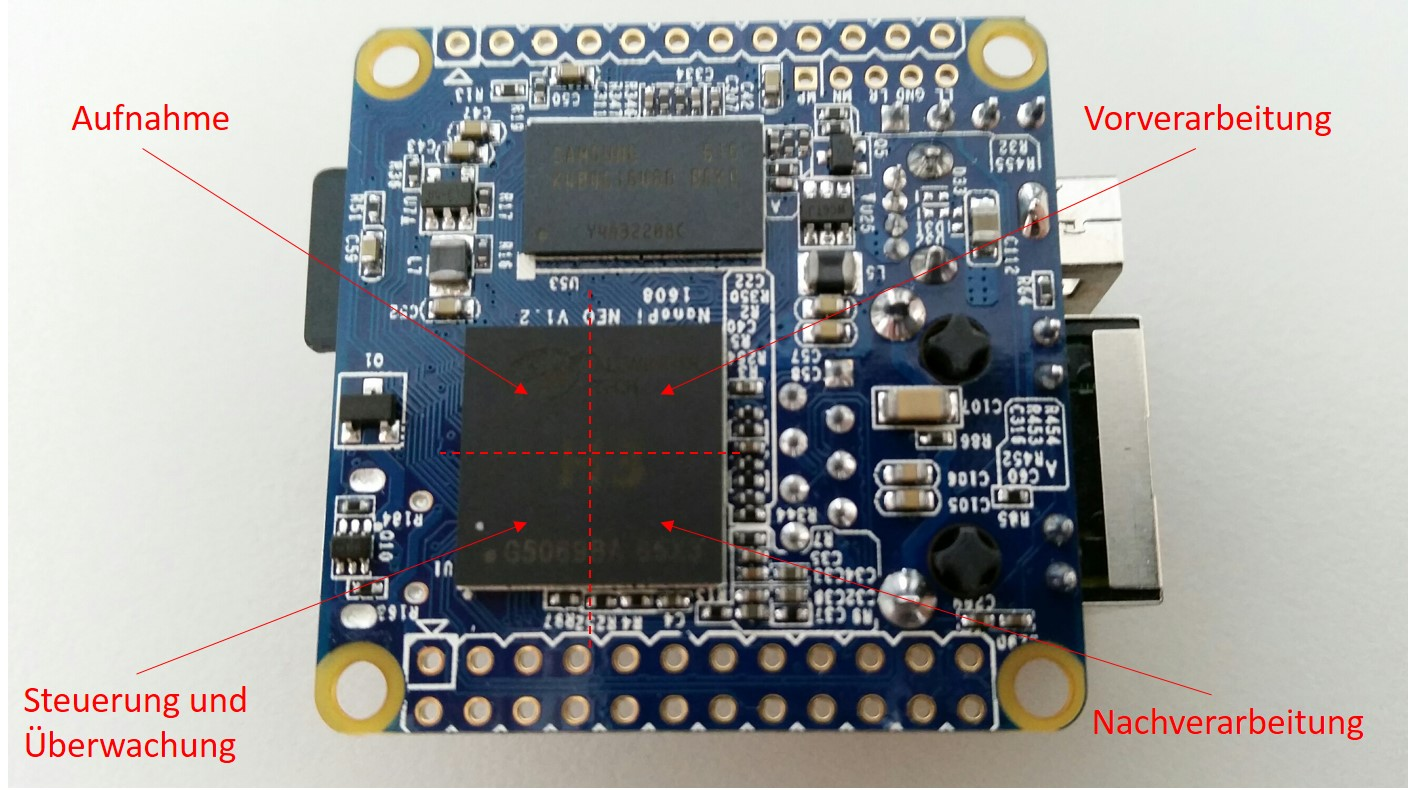
\includegraphics[height=0.49\textwidth]{Software/Architektur.jpg} 
  \caption{Aufteilung der vier Kerne.}
  \label{bArchitektur}
\end{figure}


\subsubsection{Aufnahme}
Der erste Prozess beinhaltet die Aufnahme von Videos mit der Kamera. Die Videos werden mit 25 Bildern pro Sekunde und einer Auflösung von 640x480 Pixeln aufgenommen und auf der Speicherkarte abgelegt. Dabei wird jeweils eine Videolänge von 15 Minuten erzielt, bevor es abgespeichert wird. Eine Videolänge von 15 Minuten wurde gewählt, damit nach Abschluss dieser Zeit der nächste Prozess sich schon um die Verarbeitung kümmern kann, während der Aufnahmeprozess mit dem nächsten Video beschäftigt ist. Die Videos sind im "'AVI"' Format abgespeichert und beinhalten im Durchschnitt etwa 22'500 Einzelbilder, welche vom nachfolgenden Prozess analysiert werden müssen. Mithilfe von Avconv werden diese Videos aufgenommen und mittels eines Zeitstempels, welcher Datum und Uhrzeit des Aufnahmestarts beinhaltet, im zugehörigen Ordner abgespeichert. Der Zeitstempel wird benötigt um später den Zeitpunkt eines vorbeifahrenden Verkehrsteilnehmers zu errechnen und um zu wissen, welche Videos der Reihe nach weiterverarbeitet werden müssen. Der Prozess der Videoaufnahme ist spezifisch auf den ersten der vier Prozessoren zugeteilt. Während der Aufnahmephase befindet sich dieser Kern stetig bei einer Auslastung von 95 - 100\%.

\subsubsection{Vorverarbeitung}
Sobald sich zwei Videos im zugehörigen Ordner befinden, kann davon ausgegangen werden, dass die Aufnahme des ersten Videos abgeschlossen ist. Zu diesem Zeitpunkt beginnt die Vorverarbeitung damit, die Bilder zu analysieren und diese, sobald eine Bewegung auf dem Bild erkannt wurde, in einem Ordner abzuspeichern, welcher extra für diese Frames genutzt wird. Da die Videoaufnahme innerhalb von 15 Minuten jeweils 22'500 Bilder erzeugt, muss die Vorverarbeitung etwa gleich viel Bilder in der selben Zeit auswerten können. Aus diesem Grund wurde das Programm dieses Prozesses soweit optimiert, dass nur sehr wenig einzelne Schritte durchgeführt werden müssen. Diese Analyse wird mithilfe der Bildverarbeitungs-Bibliothek OpenCV durchgeführt. Dort kann ein Video angegeben werden und daraufhin wird jeweils das nächste noch nicht genutzte Frame des Videos in eine temporäre Variable gespeichert. Mit dieser Variablen können anschliessend weitere Berechnungen durchgeführt werden. Die Vorverarbeitung nimmt jeweils zwei aufeinanderfolgenden Frames und subtrahiert dabei bei diesen Bildern jeden einzelnen Pixel an derselben Stelle voneinander ab. Falls es keine Bewegung beim spezifischen Pixel gab, so ergibt die Subtraktion der Pixel an derselben Stelle den Wert Null und somit erscheint dies auf dem Bild schwarz. Falls sich jedoch Bewegungen abgespielt haben, ergibt diese Berechnung einen höheren Wert und somit erscheint es auf dem Bild heller bzw. farbig. Dies wird für jedes der 640x480 Pixel in einem Bild durchgeführt und daraufhin werden im nächsten Schritt die erhaltenen Differenzen addiert. Somit erhält man eine Zahl, welche die Gesamtsumme aller Differenzen dieser 307'200 einzelnen Pixel repräsentiert. Diese Zahl ist schlussendlich ausschlaggebend für eine allfällige Bewegung zwischen diesen beiden Bildern. Die nachfolgende Abbildung (\fref{bFrames}) zeigt zwei aufeinanderfolgende Frames.

\begin{figure}[H]
  \centering
  \subfigure[Frame1]{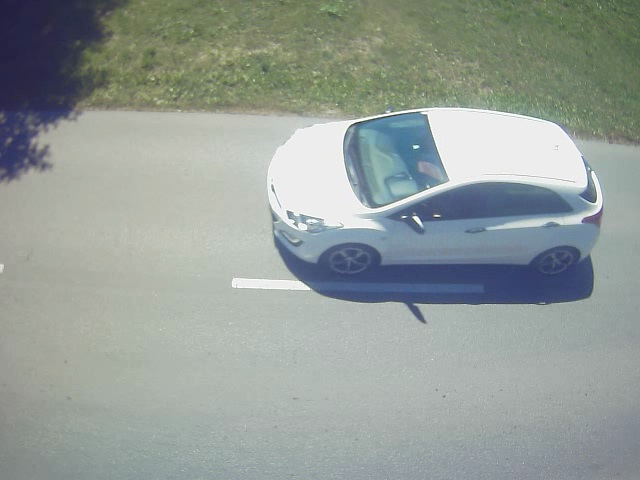
\includegraphics[width=0.40\textwidth]{Software/Frame1.jpg}}
  \subfigure[Frame2]{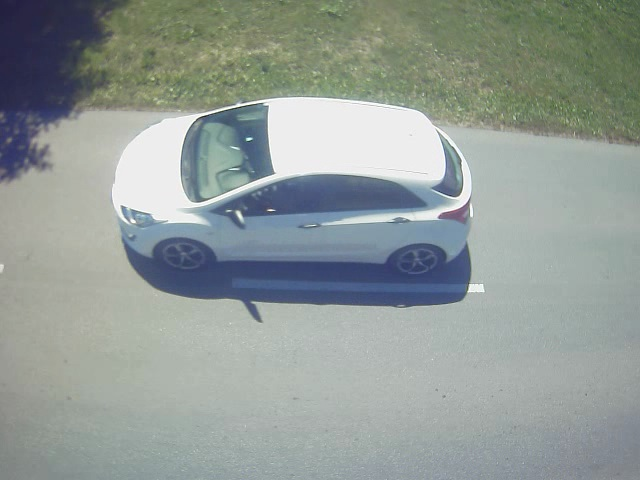
\includegraphics[width=0.40\textwidth]{Software/Frame2.jpg}}
  \caption{Zwei aufeinanderfolgende Frames}
  \label{bFrames}
\end{figure}

Anschliessend wurde die oben erwähnte Berechnung mit diesen beiden Frames durchgeführt, wodurch Bewegungen zwischen den Bildern heller bis farbig erscheinen. Das Ergebnis der Subtraktion ist im untenstehenden Bild (\fref{bBlur1}) ersichtlich.

\begin{figure}[H]
  \centering
  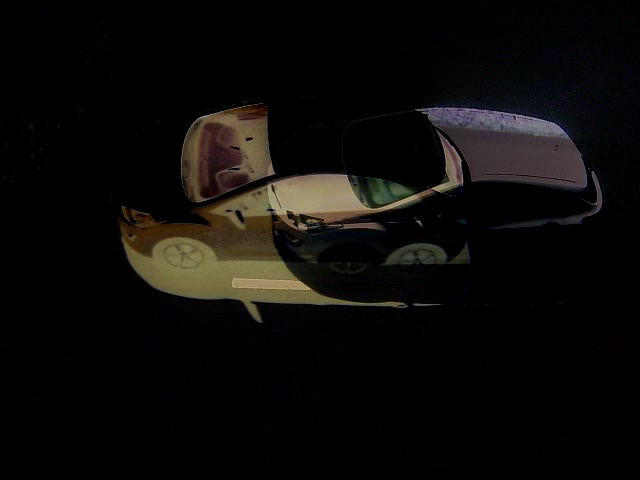
\includegraphics[height=0.3\textheight]{Software/Blur1.jpg} 
  \caption{Differenzbild der aufeinanderfolgenden Frames.}
  \label{bBlur1}
\end{figure} 

Damit ein allfälliges Rauschen oder ein vorbeilaufender Fussgänger nicht gezählt wird, wurde ein gewisser Schwellwert angegeben. Sobald die Summe der Pixel den Schwellwert überschreitet, wird das Bild temporär abgespeichert. Damit die Bilder im nächsten Schritt logisch verknüpft werden können, muss im Speichername eine Indexierung angegeben werden. Diese Indexierung ist die Zahl des Frames, welches vom Video stammt und liegt aus diesem Grund zwischen 0 und 22'499. Falls keine Speicherung stattgefunden hat wird das nächste Bild genommen und der Vorgang beginnt erneut. Mit dieser Methode werden etwa 25 Bilder pro Sekunde verarbeitet. Da jedoch das Abspeichern etwas mehr Zeit benötigt anstatt das Bild lediglich zu verwerfen, können bei höherem Verkehrsaufkommen nur etwa 20 Einzelbilder verarbeitet werden. Nachdem ein komplettes Video abgearbeitet wurde, wird es aus Platzgründen und da es für den weiteren Verlauf der Auswertung nicht mehr benötigt wird gelöscht. Dies ist die letzte Aufgabe der Vorbearbeitung, bevor danach der Prozess beendet wird und das Programm somit bereit für das nächste Video ist. Von den 22'500 Einzelbildern, die von diesem Prozess bearbeitet wurden, sind zu diesem Zeitpunkt, je nach Verkehrsaufkommen, noch etwa 500 - 1'500 Bilder im Zwischenspeicher. Diese werden danach vom nächsten Prozess, der Nachbearbeitung, weiterbearbeitet. Da die Vorverarbeitung sehr viel Leistung erbringen muss, wurden ihm die Prozessorkerne 2 und 4 zugeteilt. Die Steuerung und Überwachung, welche fix auf Prozessorkern 4 zugeteilt wurde, benötigt nicht die volle Auslastung. Aus diesem Grund kann die Vorverarbeitung mit beinahe der vollen Auslastung von zwei Kernen arbeiten und somit die vielen Einzelbilder möglichst effizient abarbeiten.

\subsubsection{Nachverarbeitung}
Nachdem die Vorverarbeitung ein Video analysiert und die relevanten Frames abgespeichert hat, kann die Nachverarbeitung damit beginnen, die Bilder weiter zu verarbeiten. Auch hier, wird der Prozess erst gestartet, wenn sich zwei unterschiedliche Ordner mit Frames im zugehörigen Ordner befinden. Somit soll gewährleistet sein, dass die Vorverarbeitung mit dem Video fertig ist, bevor die Nachverarbeitung mit dem Prozess beginnt. Das Endprodukt der Nachbearbeitung ist ein Feature Vektor. Dies ist eine Microsoft Excel Tabelle mit je einem Eintrag pro Verkehrsteilnehmer. Dabei werden möglichst viele Indikatoren pro Verkehrsteilnehmer aufgenommen und in der Tabelle abgespeichert. Je mehr Features pro Verkehrsteilnehmer gefunden werden können, desto besser kann dieser später wiedererkannt werden und somit die eigentliche Verkehrsverfolgung durchgeführt werden. Nachfolgende Tabelle (\tref{tFeatureVektor}) zeigt ein Beispiel eines Feature Vektors.

\setlength\tabcolsep{5pt}

\begin{table}[H]
\centering
\begin{tabular}{|l|l|l|l|l|l|l|l|l|l|l|l|}
\hline
\textbf{I} & \textbf{Timestamp}  & \textbf{RP} & \textbf{D} & \textbf{DC} & \textbf{CropN} & \textbf{BlurN} & \textbf{PicN} & \textbf{RX} & \textbf{RY} & \textbf{RW} & \textbf{RH} \\ \hline
1            & 18.06.17 22:55:12 & 5           & R            & 1           & crop001.tif       & blur001.tif       & pic001.tif       & 95          & 141         & 377         & 190         \\ \hline
2            & 18.06.17 22:57:19 & 8           & R            & 2           & crop002.tif       & blur002.tif       & pic002.tif       & 146         & 118         & 387         & 196         \\ \hline
3            & 18.06.17 22:57:37 & 7          & L            & 1           & crop003.tif       & blur003.tif       & pic003.tif       & 138         & 145         & 373         & 251         \\ \hline
4            & 18.06.17 22:58:10 & 7           & R            & 3           & crop004.tif       & blur004.tif       & pic004.tif       & 152         & 112         & 345         & 165         \\ \hline
5            & 18.06.17 22:59:02 & 6           & L            & 2           & crop005.tif       & blur005.tif       & pic005.tif       & 115         & 126         & 415         & 296         \\ \hline
6            & 18.06.17 22:59:23 & 5           & R            & 4           & crop006.tif       & blur006.tif       & pic006.tif       & 145         & 126         & 364         & 194         \\ \hline
7            & 18.06.17 22:59:56 & 5          & R            & 5           & crop007.tif       & blur007.tif       & pic007.tif       & 113         & 100         & 453         & 311         \\ \hline
8            & 18.06.17 22:59:59 & 9           & R            & 6           & crop008.tif       & blur008.tif       & pic008.tif       & 165         & 138         & 358         & 182         \\ \hline
9            & 18.06.17 23:00:09 & 9           & L            & 3           & crop009.tif       & blur009.tif       & pic009.tif       & 148         & 160         & 367         & 212         \\ \hline
10           & 18.06.17 23:00:18 & 7           & R            & 7           & crop010.tif       & blur010.tif       & pic010.tif       & 147         & 127         & 371         & 198         \\ \hline
11           & 18.06.17 23:00:37 & 4           & R            & 8           & crop011.tif       & blur011.tif       & pic011.tif       & 155         & 128         & 341         & 189         \\ \hline
\end{tabular}
\caption{Feature Vektor}
\label{tFeatureVektor}
\end{table}

\setlength\tabcolsep{0pt}

Der Feature Vektor zeigt den Index anhand einer fortlaufenden Nummer und den Zeitstempel, an welchem sich der Verkehrsteilnehmer in der Mitte des Kamerabildes befand. Ebenso enthält es die Information wie viele aufeinanderfolgende Bilder zu diesem Ergebnis geführt haben, in welche Richtung dieser unterwegs war und einen Zähler der sowohl für links als auch rechts fahrende Verkehrsteilnehmer stetig erhöht wird. Daneben werden im Moment noch drei Bilder abgespeichert, welche für weitere Berechnungen von Features benützt werden können. Die letzten vier Spalten zeigen die Position des Verkehrsteilnehmers im Originalbild.\\
Die Nachverarbeitung kümmert sich in erster Linie darum, den vorhandenen Feature Vektor zu öffnen und daraus relevante Informationen zu entnehmen, falls dieser vorhanden ist. Ansonsten wird ein neuer Feature Vektor generiert. Zu den relevanten Informationen gehören der Index, welcher notwendig ist, damit im Feature Vektor kein Index doppelt vorkommt und somit bereits vorhandene Bilder gelöscht werden. Zudem wird die Anzahl an Verkehrsteilnehmer, welche bis zu diesem Zeitpunkt nach links bzw. rechts gefahren sind, in einer Variablen gespeichert, damit diese beiden Zähler weiter erhöht werden können, wenn neue Verkehrsteilnehmer erkannt werden. Dies ist erforderlich, da sich dieses Programm nach Abarbeitung der Frames, welche zu einem 15-Minütigen Videos gehören, beendet und somit alle bestehenden Informationen verliert. Danach wird die Anzahl an relevanten Bildern ermittelt, welche zu einem Verkehrsteilnehmer gehören. Dies passiert, indem die Frames genommen und deren Indexierungen betrachtet werden. Falls die Indexierungen der Frames fortlaufend sind, so muss es sich um denselben Verkehrsteilnehmer handeln. Falls der Abstand zwischen zwei Frames einen gewissen Wert überschreitet, hat die Kamera für kurze Zeit keine Bewegung erkannt und somit muss es sich um einen neuen Verkehrsteilnehmer handeln. Sobald die Zahl der relevanten Bilder bekannt ist, werden diese logisch miteinander verknüpft und somit befindet sich auf diesen Frames ein Verkehrsteilnehmer, der entweder von links nach rechts oder von rechts nach links gefahren ist.\\
Mit diesen etwa 3 bis 10 Bildern, je nach Geschwindigkeit des Fahrzeugs, wird nun mithilfe der Bildverarbeitungs-Bibliothek OpenCV ein "'Blob Detection und Tracking"' durchgeführt. Hierbei werden Bewegungen zwischen zwei aufeinanderfolgenden Bildern ermittelt und somit um die Pixel in der unmittelbaren Umgebung eine konvexe Hülle gebildet, welche auch Blob genannt wird. Auf den fortlaufenden Bildern wird sich anschliessend diese konvexe Hülle immer weiter zum weiter entfernten Rand bewegen. Im Programm wurde festgelegt, was für Einschränkungen erfüllt werden müssen, damit dieser Blob als Verkehrsteilnehmer gezählt wird. Dazu gehören die Fläche der Hülle, das Verhältnis zwischen Länge und Breite, die minimale Breite und Länge und die minimale Länge der Diagonale. Falls es sich beim Blob um einen Verkehrsteilnehmer handelt, muss noch ermittelt werden, zu welchem Zeitpunkt dieser die Mitte passiert und somit die Bilder generiert werden müssen. Dies wird mithilfe einer imaginären Linie durchgeführt, welche sich in der Mitte des Bildes befindet. Da die Position des Blobs von Anfang an bekannt ist, kann somit auch ermittelt werden, ob der Verkehrsteilnehmer von links nach rechts oder von rechts nach links gefahren ist.\\
Nachfolgende Abbildungen (\fref{bMotionDetection}) zeigt ein Auto, welches von rechts nach links fahrend von der Kamera mit drei Frames aufgenommen wurde. Da dieses Auto alle festgelegten Parameter erfüllt, wird es als Verkehrsteilnehmer erkannt und eine konvexe Hülle gebildet. Die konvexe Hülle wird immer um zwei nachfolgende Frames gebildet, weshalb diese bei sämtlichen Bildern länger ist wie der entsprechende Verkehrsteilnehmer. In Frame 1 und 2 befindet sich die Mitte der konvexen Hülle und somit auch die Mitte des gelben Quadrats jeweils auf der rechten Seite der Linie, weshalb zu diesem Zeitpunkt noch keine Zählung durchgeführt wurde. Erst bei Frame 3 hat die Mitte des Blobs die rote Linie überquert und somit wurde die Funktion zum Abspeichern eines Fahrzeugs und generieren eine Zeile im Feature Vektor ausgelöst.

\begin{figure}[H]
\centering
	\subfigure[Blob Frame 1]{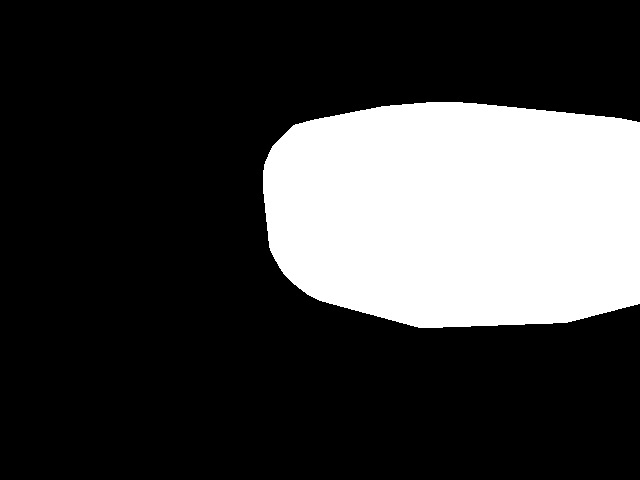
\includegraphics[scale=0.32]{Software/Blob1.jpg}}\quad
   \subfigure[Bild Frame 1]{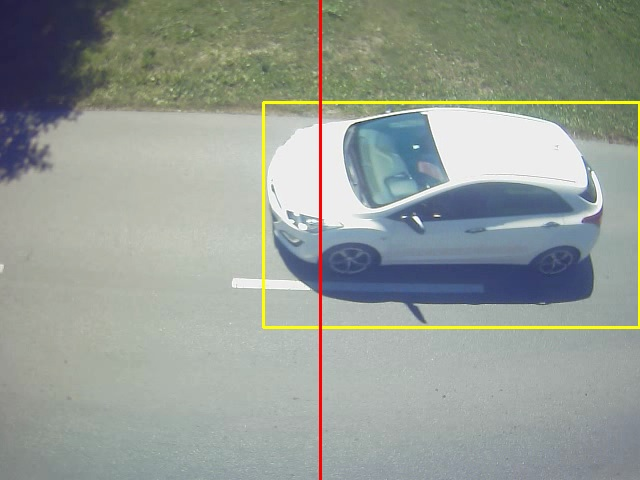
\includegraphics[scale=0.32]{Software/Detection1.jpg}}\\
   \subfigure[Blob Frame 2]{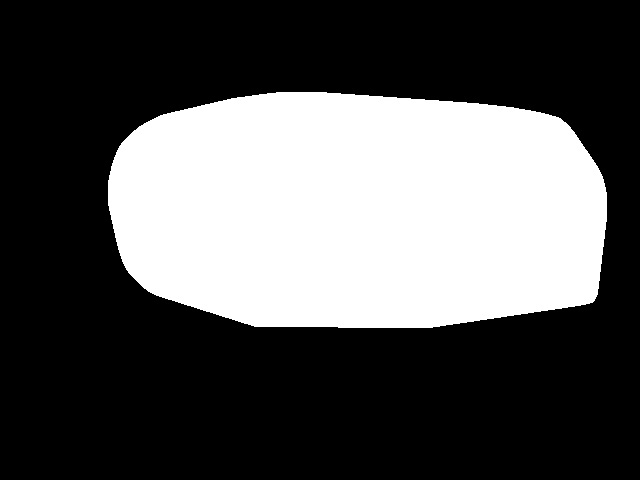
\includegraphics[scale=0.32]{Software/Blob2.jpg}}\quad
   \subfigure[Bild Frame 2]{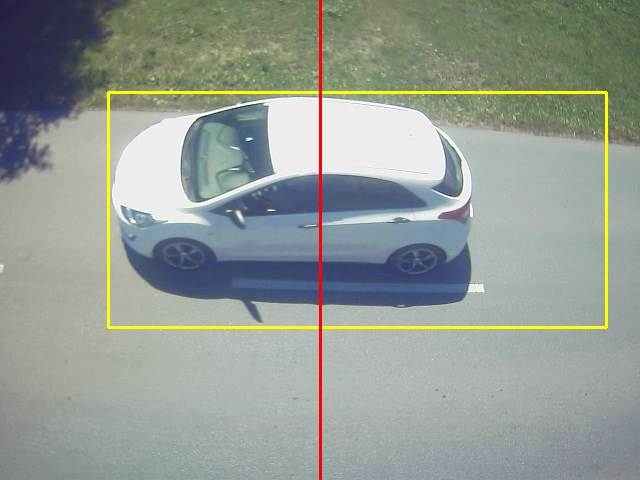
\includegraphics[scale=0.32]{Software/Detection2.jpg}}\\
   \subfigure[Blob Frame 3]{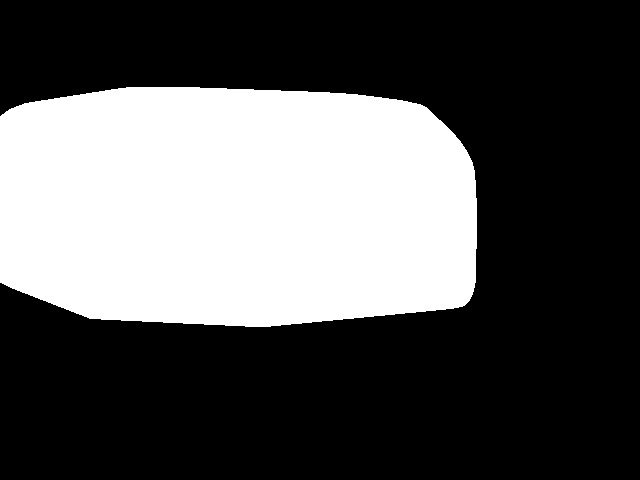
\includegraphics[scale=0.32]{Software/Blob3.jpg}}\quad
   \subfigure[Blob Frame 3]{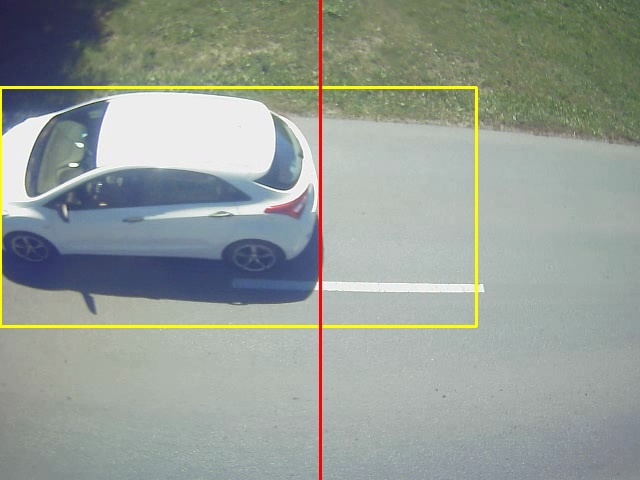
\includegraphics[scale=0.32]{Software/Detection3.jpg}}
\caption{Vehicle Tracking mithilfe von Blobs}
\label{bMotionDetection}
\end{figure}

In der Funktion zur Speicherung werden die drei vorgängig erwähnten Bilder in den entsprechenden Ordner im Speicher abgelegt und schlussendlich alle relevanten Informationen an den Filehandler übergeben. Dieser öffnet die Datei des Feature Vektors und schreibt alle Informationen inklusive generierten Zeitstempel in eine neue Zeile.\\
Danach ist dieser Verkehrsteilnehmer erfolgreich aufgenommen und somit abgeschlossen und der Nächste kann ermittelt werden.
Wenn sich keine Bilder mehr im Frames Ordner befinden, beginnt die letzte Aufgabe dieses Programms. Dies bedeutet, den eben bearbeiten Ordner zu löschen, da auch dieser für die weitere Auswertung nicht mehr benötigt wird. Der Nachbearbeitung wurde fix der Prozessorkern 3 zugeteilt. Bei hohem Verkehrsaufkommen benötigt diese auch die vollen 100\% dieses Kerns. \cite{OpenCVCC}

\subsubsection{Steuerung und Überwachung}
Da sich die vorhin erwähnten Prozesse selber beenden, sobald ihre Arbeit erledigt ist, benötigt es einen Prozess, welcher sich um die Koordination kümmert. Dies ist auch die Hauptaufgabe dieses Prozesses. Videos werden nur zwischen morgens um 05:00 Uhr und abends um 21:00 Uhr aufgenommen. Dies ist notwendig um sicherstellen zu können, dass alle Videos bis zum nächsten Morgen abgearbeitet sind. Somit soll ein Speicherplatz Problem verhindert werden, falls die Vorverarbeitung aufgrund von hohem Verkehrsaufkommen die Videos langsamer prozessiert als diese aufgenommen werden.\\
Die Steuerung und Überwachung ist so konzipiert, dass sie ständig eine Schleife von Befehlen durchführt. Die erste Aufgabe darin ist es zu prüfen wie spät es im Moment ist. Falls die Nachtphase noch nicht aktiv ist wird kontrolliert, ob der Prozess zur Videoaufnahme noch läuft. Damit kann sofort ein neuer Prozess zur Aufnahme gestartet werden, falls kein Video mehr aufgenommen wird.\\
Als nächstes wird die Anzahl Videos im dazugehörigen Ordner kontrolliert und anschliessend auch hier der Prozess zur Vorverarbeitung analysiert. Wenn die Vorverarbeitung nicht läuft, muss diese neu gestartet werden. Dazu wird jedoch der Pfad zum Video benötigt, welches als nächstes bearbeitet werden muss. Aus diesem Grund muss der Pfad anhand des Erstellungsdatums der Videos herausgelesen werden. Danach kann die Vorverarbeitung mit dem dazugehörigen Pfad des Videos gestartet werden.\\
Nach dem gleichen Konzept geht es auch beim dritten Prozess, der Nachbearbeitung, weiter. Der einzige Unterschied zwischen dem zweiten und dritten Prozess besteht darin, dass hier der Pfad zum Ordner mit den Frames benötigt wird, um die Nachverarbeitung zu starten.\\
Da daneben noch ein Webserver läuft, um Informationen bereitstellen zu können, wenn man sich mit dem Fast and Curious Gerät verbindet, hat die Steuerung und Überwachung noch kleinere Aufgaben für diesen Webserver. Dies beinhaltet, auf Eingaben der Website zu reagieren und Ordner zu erstellen oder verschieben, wenn dies vom Benutzer gewünscht ist. Zudem ist eine Temperaturüberwachung eingebaut. Aus diesem Grund wird einmal pro Minute die Kerntemperatur ausgelesen und in ein File geschrieben. Diesem Prozess wurde der Prozessorkern 4 zugeteilt. Da die Auslastung des Scripts jedoch nicht sonderlich hoch ist, teilt sich dieser Prozess den Kern mit der Vorverarbeitung. \cite{Bash}